\section{Značaj podataka u dubokom učenju}
Prvi i najdulji praktični korak treninga predstavlja priprema podataka. 
Sve ovisi o zadatku koji mreža mora riješiti, ali, generalno je pravilo da je više podataka bolje.
Konačna kvaliteta rješenja osim o arhitekturi mreže koju dizajniramo, ovisi o kvaliteti podataka kojom ju usmjeravamo.
Priprema podataka vrši se u 3 glavna koraka \cite{generalDatasets}:
\begin{enumerate}
\item Prikupljanje
\item Klasifikacija
\item Označavanje
\end{enumerate} 
\subsubsection{Prikupljanje podataka}
Prikupljanje podataka mora biti sustavan i smislen proces jer može otežati i olakšati daljnje korake. 
Najpreporučeniji način za prikupljanje je dugoročno i postepeno spremanje podataka jer rezultira velikim brojem objektivnih i kvalitetnih podataka.
Odlučeno je koristiti metodu računalnog generiranja vlastitog skupa podataka. 
Razlog tome je raznolikost elemenata koje mreža mora moći detektirati i fleksibilnost koju dobivamo jednom kada ustanovimo sve potrebe.
\subsubsection{Klasifikacija i označavanje podataka}
Generirani podaci na određeni način moraju biti prikazani mreži. 
Iako u mrežu slika ulazi kao vektor dimenzija \texttt{(visina x širina x kanali)}, mreži su potrebni i podaci za uspoređivanje rezultata i računanje uspješnosti.
U ovom radu koristi se \texttt{.csv} datoteka za dohvaćanje i kao opisnik slika. 
Postupak automatskog generiranja slika uvelike je olakšao klasifikaciju i označavanje jer je cijeli postupak ostvaren kao "cjevovod".
Pri izlasku, slika bi bila prikazana kao na slici ~\ref{fig:pipelineExitExample}.
Datoteka bi upisano imala ime slike, simbol na slici, širinu, visinu i točan položaj elementa na slici. 
Prednost ovog pristupa je i u tome što slika nije zadana apsolutnom putanjom, što znači da su slike mogle biti kreirane na vlastitom računalu, prenešene na udaljeni server za treniranje i bez komplikacija biti korištene. \\
Veličina opisnika je također bila zanemariva. \\ 
Nakon raspodjele \texttt{80:20} za trening i validaciju na 15 000 slika, veličine su bile \texttt{440kB} i \texttt{110kB} dok je direktorij sa slikama bio veličine \texttt{6,7GB}.

\begin{figure}[h!]
	\centering
	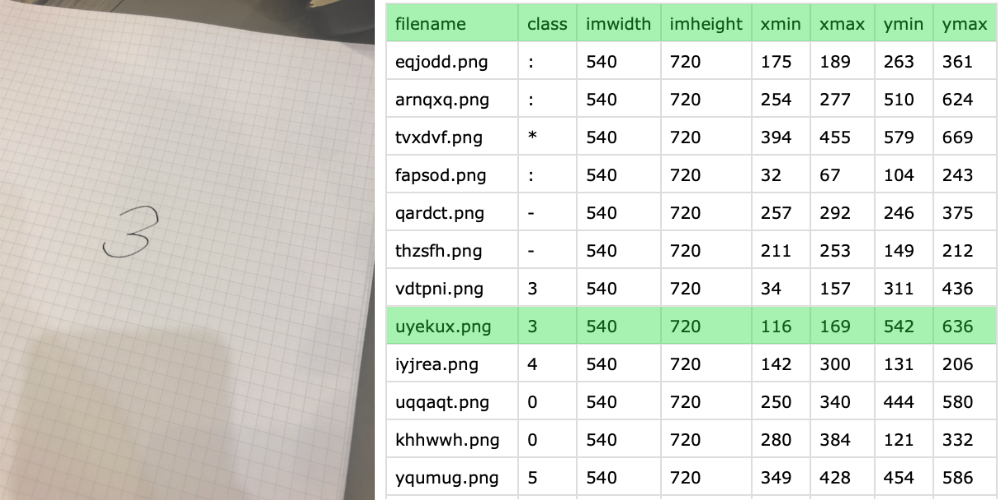
\includegraphics[width=1.0\linewidth]{image_csv}
	 \caption{Slika i pripadajuća referenca u .csv datoteci}
 	 \label{fig:pipelineExitExample}
\end{figure}

\section{Generiranje slika}
\subsection{Generalizacija postupka}
Za relativan uspjeh treniranja mreže za detekciju i klasifikaciju 14 tekstovnih elemenata (0-9, +, -, *, :) rezultati su pokazali da je potrebno minimalno 10 000 slika. 
Ne samo zbog broja elemenata već i zbog složenosti i raznolikosti između njih. 
Razvijeni postupak primjenjuje sve taktike \cite{chollet2017deep} potrebne za stvaranje raznovrsnog i kvalitetnog skupa podataka.
Zbog transformacija opisanih u daljnjim dijelovima poglavlja, gotovo je nemoguće, da iako se isti font stavlja na pozadinu, nastane isti oblik.
Na slici ~\ref{fig:imageGenerationPipeline} prikazana je topologija cjevovoda koja kreira slike.
Cijeli cjevovod implementiran je unutar programskog paketa \emph{ImageGenerator}, razvijen u svrhu apstraktiranja cijelog postupka.
\begin{figure}[h!]
	\centering
	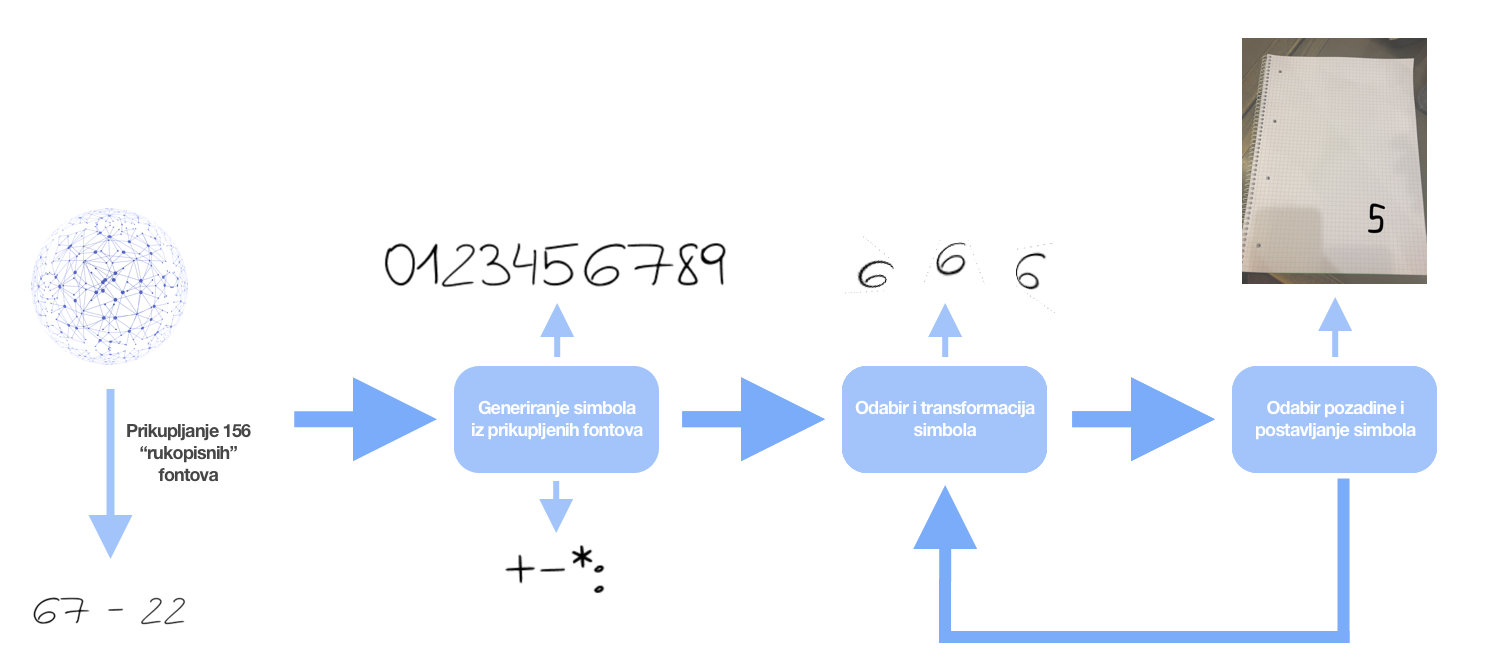
\includegraphics[width=1.0\linewidth]{image_generation_pipeline}
	 \caption{Prikaz visoke razine cjevovoda za generiranje slika}
 	 \label{fig:imageGenerationPipeline}
\end{figure}

\subsection{Prikupljanje fontova}
Ispisivanje velikog broja simbola sa razlikom između varijacija istog monoton je i neisplativ posao, posebice zbog dostupnosti svih potrebnih resursa na internetu.
U prilog je također išlo to što su dostupni fontovi, koji primjenjuju rukopisni stil, najčešće zbilja napisani rukom i vektorizirani, pa generiranje i transformiranje neće negativno utjecati na kvalitetu.
Osim rukopisnih fontova, prikupljen je i mali broj fontova koji su stilski između čistog rukopisnog i tipkanog. \\
Fontovi su bili prikupljeni sa sljedećih izvora, a na slici ~\ref{fig:fontDiffs} vidljivi su primjeri istih:
\begin{itemize}
\item \url{https://www.dafont.com}
\item \url{https://www.1001fonts.com}
\item \url{https://www.1001freefonts.com}
\end{itemize}
\begin{figure}[h!]
	\centering
	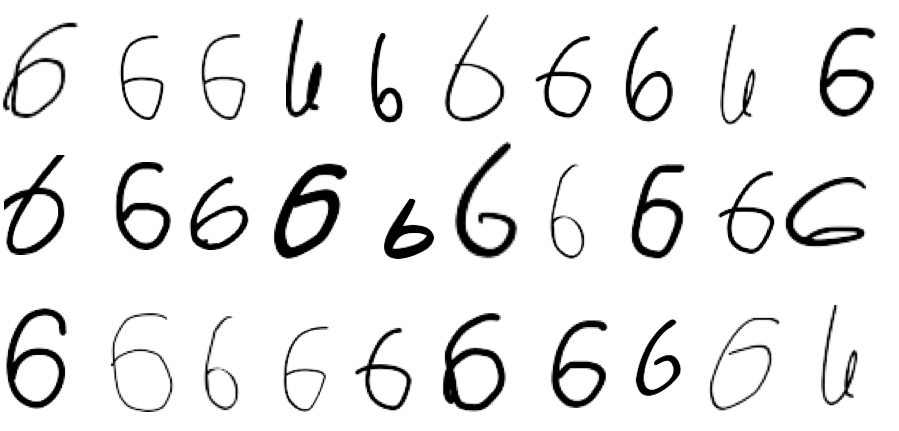
\includegraphics[width=0.85\linewidth]{font_diffs}
	 \caption{Varijacije unutar simbola uzrokovane fontovima}
 	 \label{fig:fontDiffs}
\end{figure}

\subsection{Generiranje simbola}
Nakon prikupljanja i sortiranja fontova, generiranje samih simbola jednostavan je posao.
Važno je očuvati transparentnost pozadine iza simbola jer u trenutku kada se postavi na pozadinu po izboru, ona mora biti vidljiva.
Nakon postavljanja simbola, izvode se transformacije opisane u daljnjem tekstu.
\subsection{Transformacije}
Prije postavljanja simbola na nasumično odabranu sliku, svaki simbol prošao je kroz tri točke transformiranja:
\begin{enumerate}
\item Skaliranje
\item Rotacija
\item Afina transformacija
\end{enumerate}
Cilj transformacija je maksimalno unijeti raznolikost unutar skupa podataka u slučaju premalog ili presličnog broja slika.
Klasa \emph{ImageGenerator} za to se brine na sličan način kao programski paket \emph{Keras.preprocessing.image.ImageDataGenerator} \cite{Keras.io}.
Transformacije nad slikama izvedene su pomoću programskog paketa \emph{OpenCV} \cite{OpenCV} jer apstraktira potrebne matematičke operacije na razumljiv, lako koristiv i prilagodljiv način.
Tijekom faze transformiranja i postavljanja slike na pozadinu, one su u obliku matrice definirane pomoću programskog paketa \emph{Numpy}.
\subsubsection{Skaliranje}
Skaliranje pomoću \emph{OpenCV} paketa može se izvoditi ili ručno, specifirajući točnu veličinu, ili dajući faktor skaliranja.
\emph{OpenCV} također automatski primjenjuje \emph{interpolaciju} kako bi se kvaliteta maksimalno sačuvala.
Skaliranje se izvodi na način da se matrica slike pomnoži sa matricom skaliranja, zadanom na sljedeći način:
$$
M
=
\begin{bmatrix}
	s_{x} & 0 \\
	0 & s_{y}
\end{bmatrix},
$$
gdje je $s_{x}$ faktor skaliranja u $x$ dimenziji, a $s_{y}$ faktor skaliranja u $y$ dimenziji.
Rezultat skaliranja vidljiv je na slici ~\ref{fig:scaling}
\lstset{numbers=left}
\lstinputlisting[language=python]{CodeSamples/Scaling.py}
\begin{figure}[h!]
	\centering
	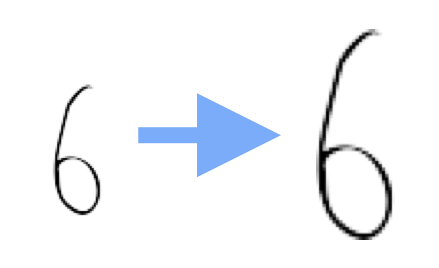
\includegraphics[width=0.4\linewidth]{Scaling}
	 \caption{Rezultat primjene skaliranja uz faktore $s_{x} = s_{y} = 1.25$}
 	 \label{fig:scaling}
\end{figure}
\subsubsection{Rotacija}
Rotacija slike za kut $\theta$ ostvaruje se množenjem s matricom rotacije:
$$
M
=
\begin{bmatrix}
	\cos(\theta) && -\sin(\theta) \\
	\sin(\theta) && \cos(\theta)
\end{bmatrix}
$$
Iako je rotiranje izvedeno iz središnje točke, \emph{OpenCV} nudi podršku za eksplicitno zadavanje točke oko koje će se rotacija izvoditi.
Rezultat rotiranja vidljiv je na slici ~\ref{fig:Rotating}.
\lstset{numbers=left}
\lstinputlisting[language=python]{CodeSamples/Rotation.py}
\begin{figure}[h!]
	\centering
	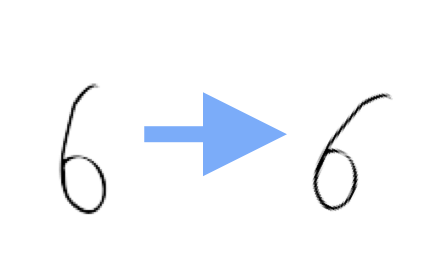
\includegraphics[width=0.4\linewidth]{Rotation}
	 \caption{Rezultat primjene rotacije s $\theta = 25$}
 	 \label{fig:Rotating}
\end{figure}
\subsubsection{Afine transfromacije}
Afine transformacije koristimo za prividno transformiranje simbola "u prostoru", bez velikog rizika od prevelike distorzije slike jer, sve paralelne linije nakon transformacije ostaju paralelne.
\emph{OpenCV} afinu transformaciju vrši tako da tri odabrane točke na slici pomakne za određeni koeficijent.
Kao i ostale transformacije, matematički nastaje množenjem matrice slike s matricom afine transformacije oblika:
$$
\begin{bmatrix}
	1 && \tan(\beta) \\
	\tan(\alpha) && 1
\end{bmatrix} ,
$$
gdje su $\alpha$ i $\beta$ razlike u kutevima prema pripadajućim koordinatnim osima.
Rezultat primjene afine transformacije na simbolu vidljiv je na slici ~\ref{fig:Affine}
\lstset{numbers=left}
\lstinputlisting[language=python]{CodeSamples/Affine.py}
\begin{figure}[h!]
	\centering
	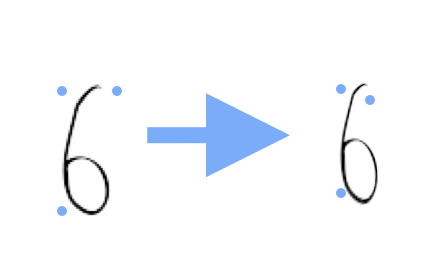
\includegraphics[width=0.4\linewidth]{Affine}
	 \caption{Rezultat primjene afine transformacije s pripadajućim referentnim točkama}
 	 \label{fig:Affine}
\end{figure}

\subsection{Kreiranje cjelovitih slika}
Kreiranje cjelovitih slika svodilo se na postavljanje generiranih i transformiranih simbola na pozadinu po izboru.
Pozadina također igra veliku ulogu u prepoznavanju jer mreža pregledava cijelu sliku.
Za potrebe ovog rada izabrana je pozadina matematičkih bilježnica uz pretpostavku da bi se iste najčešće koristile kada bi se naučena mreža koristila u stvarnom svijetu.
Izlazi iz mreže vidljivi su na slikama ~\ref{fig:ImageGeneratorOutputs} i ~\ref{fig:ImageGeneratorTermOutputs}.
Slike su spremljene u direktorij \texttt{Images}, a \texttt{.csv} opisnik u direktorij \texttt{Data} odakle će se dalje referencirati za kreiranje \texttt{.record} datoteke za daljnje korištenje \emph{Tensorflow-u}.
\begin{figure}
	\subfloat[Izlazna slika iz \emph{ImageGenerator-a}] {%
		
\includegraphics[width=0.4\linewidth]{image_generator_output} %
		\label{fig:ImageGeneratorOutputs}
	}

	\subfloat[Ispis za praćenje statusa generiranja slika] {%
		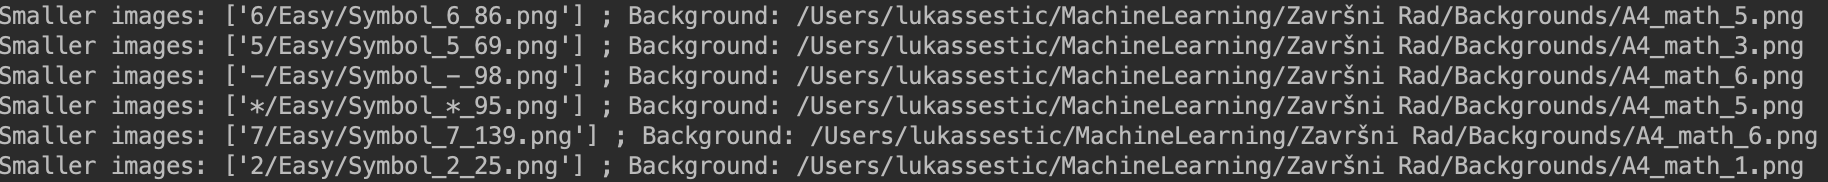
\includegraphics[width=1.0\linewidth]{image_generator_term_output} %
		\label{fig:ImageGeneratorTermOutputs}
	}
\end{figure}

\section{TFRecords}
Zašto je bolje za mrežu da podatke čita iz \texttt{.record} datoteke nego odvojeno slike i pripadajuće opise?
Zamislimo sljedeći scenarij.
Učenje se izvodi na računalu sa \texttt{HDD} diskom, slike i oznake su u različitim direktorijima.
Svako čitanje sljedeće slike i oznake rezultira potencijalnim pomicanjem glave diska.
Cilj je da sve potrebne datoteke budu što bolje poravnate u memoriji.
Tu se pokazuje najveći značaj \emph{TFRecords} datoteke. 
Jedna binarna datoteka koja sadrži sve informacije za mrežu, jedinstveno poravnata u memoriji \cite{TFRecords}. \\
U pozadini, \emph{TFRecords} je format koji koristi \emph{Protocol buffer} tehnologiju.
\emph{Protocol buffer} ili kraće \emph{Protobuf} je knjižnica za efikasnu serijalizaciju strukturiranih podataka (\cite{tensorflow.org}).
Konkretno, koristimo \emph{Protobuf} poruke oblika \texttt{"string" : value} za predstavljanje objekata mreži.
U mom slučaju, slike su zapisane na sljedeći način:
\begin{itemize}
\item height = \texttt{int64}
\item width = \texttt{int64}
\item filename = \texttt{bytes}
\item sourceid = \texttt{bytes}
\item encoded = \texttt{bytes}
\item format = \texttt{bytes}
\item xmins = \texttt{float\_list}
\item xmaxs = \texttt{float\_list}
\item ymins = \texttt{float\_list}
\item ymaxs = \texttt{float\_list}
\item classes\_text = \texttt{bytes\_list}
\item classes = \texttt{int64\_list}
\
\end{itemize}
Svi navedeni podaci zapisuju se pod ključ \texttt{feature}. \\
Kako u našem slučaju vršimo detekciju i klasifikaciju objekata, bitno je da na neki način i klasama damo jedinstveni identifikator.
Naime, u \emph{TFRecords} datoteku pod ključ \emph{classes} koji sadrži podatke o tom koji su svi objekti na slici ne pišemo doslovno ime objekta (npr. automobil, kuća, ...).
Pišemo brojčanu vrijednost istog objekta koja ga predstavlja. 
Isti način je precizniji i sažetiji. \\
Primjerice, ime dnevnika koji sadrži mapiranja iz objekta u njegovu brojčanu vrijednost naziva se \emph{Label map} i osim za stvaranje \emph{TFRecords} datoteke, koristi ga i sama mreža i mi kad iz mreže čitamo što je ista prepoznala.
Za kreiranje datoteke praćeni su koraci opisani na službenoj \emph{Tensorflow} stranici.
